% \section{Proof of Lemma \ref{lem:lower-bound}}
% \label{appendix:lower-bound}
% \begin{proof}
% Let $N = {n \choose 2}$ be the maximum possible number of edges in a graph. The number of undirected unweighted graph on $n$ vertices and $\frac{m}{3}$ edges is given by  ${N \choose \frac{m}{3}}$. Clearly, this number will be less than than the number of undirected unweighted graphs on \textit{atmost} $m$ edges. Now,
% \begin{equation}
%     \begin{split}
%         \nonumber
%         {N \choose \frac{m}{3}} &= \frac{N (N -1)...(N -(\frac{m}{3}-1))}{\frac{m}{3}!}\\
%         &\geq (3.\frac{N +1}{m} - 1)^{\frac{m}{3}}\\
%         &\geq 2^{\frac{m}{3}} \;\;\;\text{( Since $\frac{N +1}{m} > 1$)}
%     \end{split}
% \end{equation} 
% Since there are at least $2^{\frac{m}{3}}$ undirected unweighted graph on $n$ vertices and atmost $m$ edges, we will require $\Omega(m)$ space for storing at least one such graph. Hence, proved.
% \end{proof}


\section{Comparison of Query Time with Static Algorithms}
\label{appendix:non-trivial-query-time}
Goldberg and Rao \cite{DBLP:conf/focs/GoldbergR97a} gave a deterministic algorithm for computing $(s,t)$-mincut in an undirected unweighted graph that runs in ${\cal O}(n^{3/2}m^{1/2})$ time. Karger and Levine \cite{DBLP:conf/stoc/KargerL98} gave an algorithm that runs in ${\cal O}(nm^{2/3}c_{s,t}^{1/6})$ time for the same problem. 

We show that the query time of our data structure is ${\Omega}(\sqrt{n})$ times faster than both of them. The query time we achieve is ${\cal O}(\min(m,nc_{s,t}))$.
It is clear that $\frac{n^{3/2}m^{1/2}}{m}\geq \sqrt{n}$ and thus, the query time is $\Omega(\sqrt{n})$ times faster than Goldberg and Rao's algorithm \cite{DBLP:conf/focs/GoldbergR97a}. We can show the same for Karger and Levine's algorithm \cite{DBLP:conf/stoc/KargerL98} by separately considering the cases $m<nc_{s,t}$ and $m\geq nc_{s,t}$. Recently, Liu and Sidford \cite{DBLP:journals/corr/abs-2003-08929} gave a deterministic algorithm for computing $(s,t)$-mincut on unweighted graphs in ${\cal O}(m^{4/3 + o(1)})$ time.

% \section{Proof of Lemma \ref{lem:3-vertex-lemma} (3-vertex lemma)} \label{appendix:3-vertex-lemma}

% \begin{proof}
% Let $\alpha = c(\bar{A}\cap B, A\cap {B}),
% ~\beta = c(\bar{A} \cap B, A\cap \bar{B}),~\gamma=c(\bar{A} \cap B, \bar{A}\cap \bar{B})$.
% Refer to Figure \ref{fig:non-S-crossing} (i) that illustrates these edges and the respective cuts.
% \begin{figure}[H]
% \centering
% 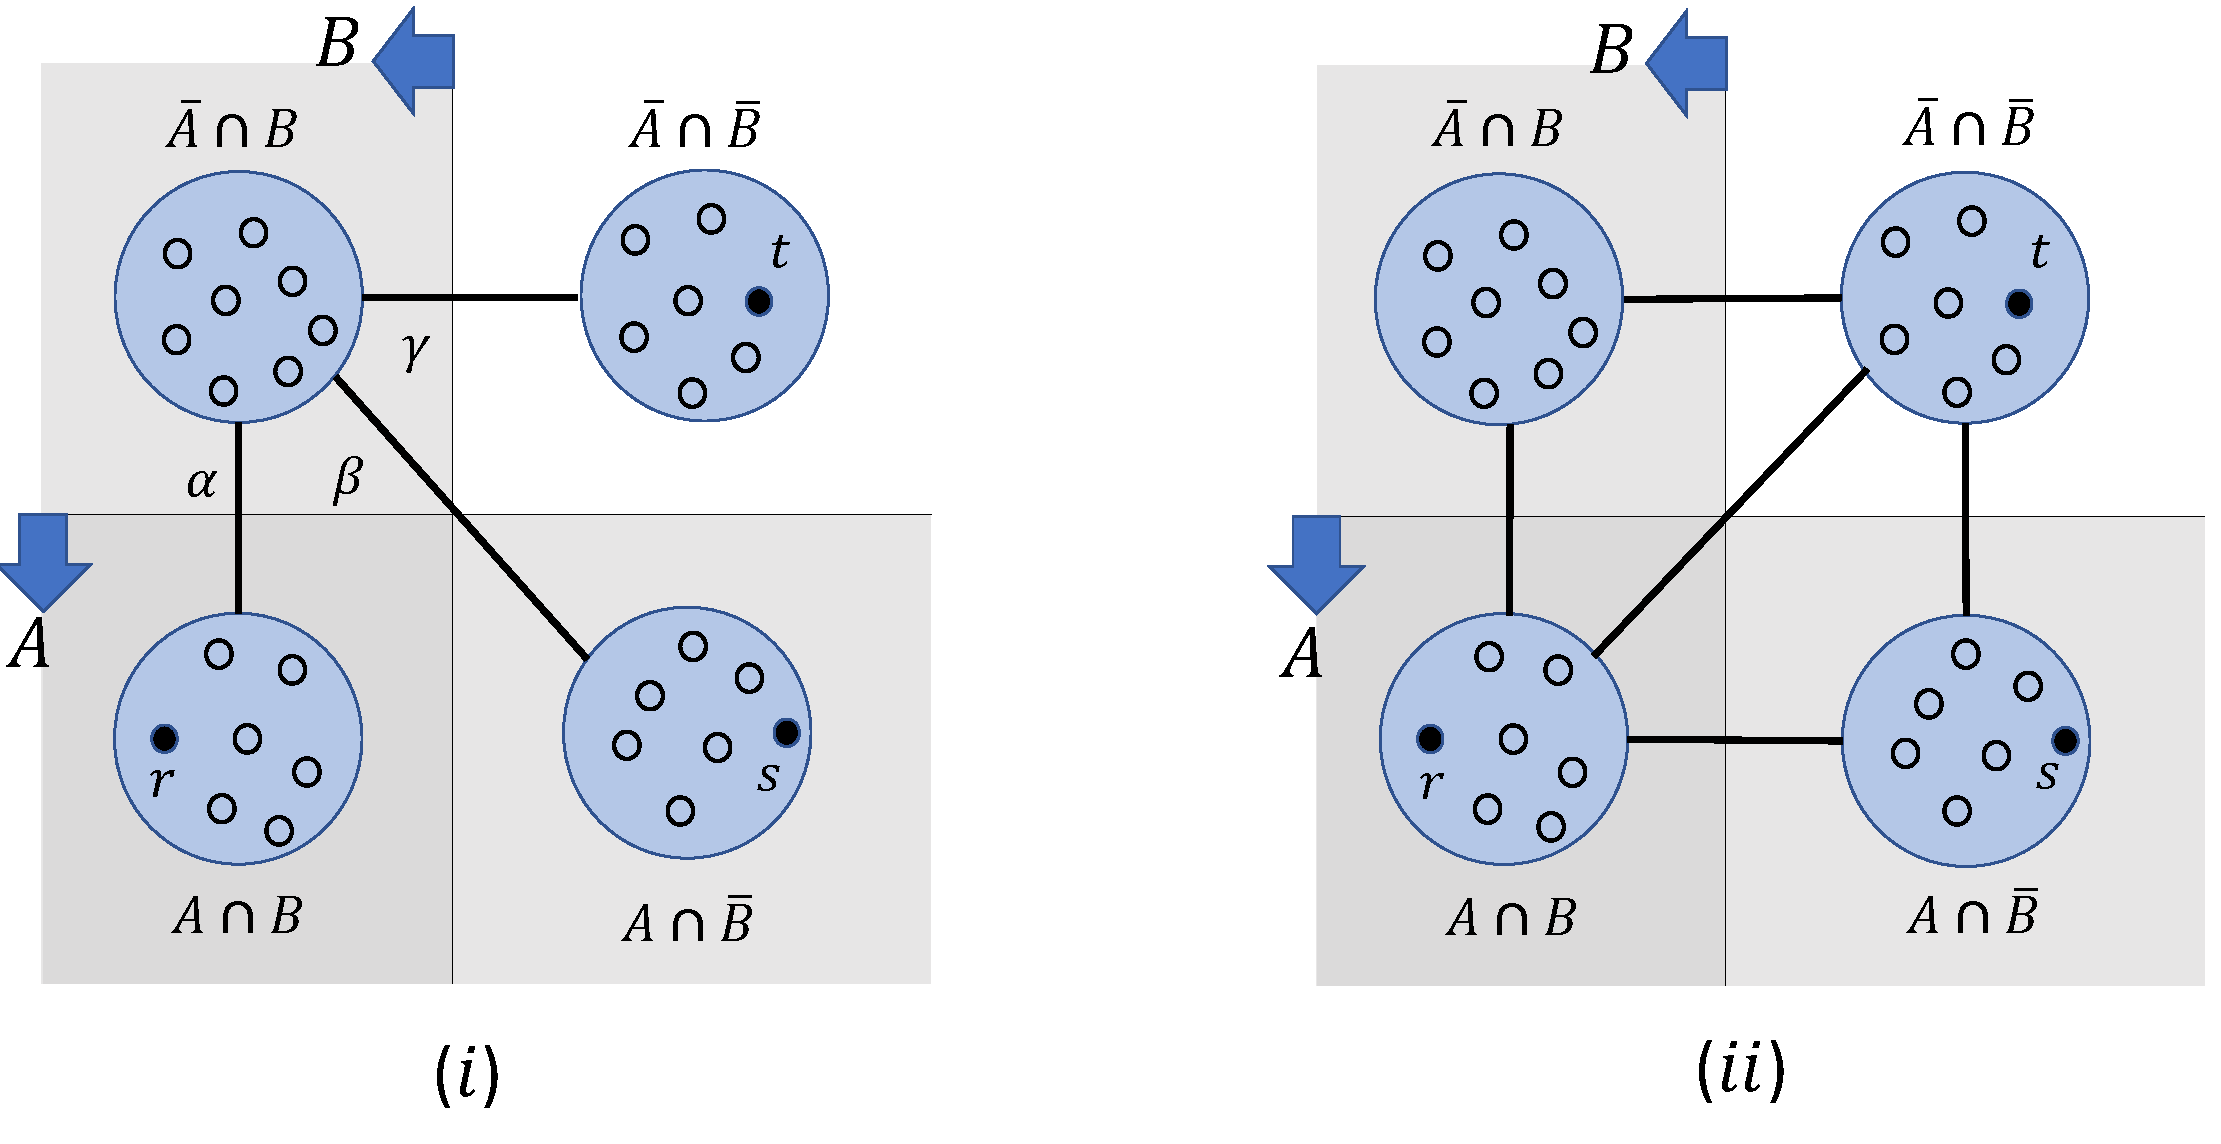
\includegraphics[width=0.75\textwidth]{src/images/S-crossing-and-non-crossing_new.pdf}
%     \caption{(i) $\alpha$, $\beta$ and $\gamma$ denote the capacities of edges incident on $\bar{A}\cap B$ from $A\cap B$, $A\cap \bar{B}$, and $\bar{A} \cap \bar{B}$ respectively. (ii) There are no edges along the diagonal between $\bar{A}\cap {B}$ and $A\cap \bar{B}$.}
% \label{fig:non-S-crossing}
% \end{figure}

% Applying Lemma \ref{lem:subset-property-of-min-cut}
% on $(s,t)$-mincut with $S=A$ and $S'= \bar{A}\cap B$, we get
% \begin{equation}
%     \alpha + \beta \le \gamma 
% \label{eq:alpha+beta-le-gamma}
% \end{equation}
% Applying Lemma \ref{lem:subset-property-of-min-cut} on $(r,s)$-mincut with $S=\bar B$ and  $S'= \bar{A} \cap B$, we get $\gamma + \beta \le \alpha$. This inequality combined with Inequality \ref{eq:alpha+beta-le-gamma} implies that $\beta=0$. That is, $c(\bar{A}\cap B, A\cap \bar{B})=0$. This completes the proof of Assertion (1). Refer to Figure \ref{fig:non-S-crossing} (ii) for an illustration. 
% It follows from (1) that $\alpha=\gamma$.
% That is, $\bar{A} \cap B$ has equal number edges incident from $\bar{A}\cap \bar{B}$ as from $A\cap B$.  This fact can be easily used to infer Assertions (2) and (3) by 
% removing $\bar{A}\cap B$ from $B$ and
% $\bar{A}$ respectively.
% \end{proof}

% \section{Compact representation for all global mincuts} \label{appendix:cactus}

% Let $c_V$ denote the value of the global mincut of the graph $G$.
% Dinitz, Karzanov, and Lomonosov \cite{DL76} showed that there exists a graph ${\cal H}_V$ of size $O(n)$ that compactly stores all global mincuts of $G$. 
% %In order to maintain the distinction between the two graphs,
% Henceforth, we shall use nodes and structural edges for vertices and edges of ${\cal H}_V$ respectively. There exists a projection mapping $\pi:V(G)\rightarrow V({\cal H}_V)$ assigning a vertex of graph $G$ to a node in graph ${\cal H}_V$. In this way, any cut $(A,{\bar A})$ in cactus ${\cal H}_V$ is associated to a cut $(\pi^{-1}(A),\pi^{-1}(\bar A))$ in the original graph $G$.
% The graph ${\cal H}_V$ has a nice tree-like structure with the following properties.
% \begin{enumerate}
%     \item Any two distinct simple cycle of ${\cal H}_V$ have at most a node in common. This is equivalent to the property that each structural edge of ${\cal H}_V$ belongs to at most one simple cycle. Each cut in ${\cal H}_V$ either corresponds to a tree edge or a pair of cycle edges in the same cycle.
%     \item If a stuctural edge belongs to a simple cycle, it is called a \textit{cycle edge} and its weight is $\frac{c_V}{2}$. Otherwise, the structural edge is called a \textit{tree edge} and its weight is $c_V$.
%     \item For any cut in the cactus ${\cal H}_V$, the associated cut in graph $G$ is a global mincut. Moreover, any global mincut in $G$ must have at least one associated cut in ${\cal H}_V$.
% \end{enumerate}

% Let $\nu$ and $\mu$ be any two nodes in the cactus ${\cal H}_V$. If they belong to the same cycle, say $c$, there are two paths between them on the cycle $c$ itself - their union forms the cycle itself. Using the fact that any two cycles in  ${\cal H}_V$ can have at most one common node, it can be seen that these are the only paths between $\nu$ and $\mu$. Using the same fact, if $\nu$ and $\mu$ are two arbitrary nodes in the cactus, there exists a unique path of cycles and tree edges between these two nodes. Any global mincut that separates $\nu$ from $\mu$ must correspond to a cut in this path.

% \subsection*{Construction of $(s,t)$-strip from cactus}
% \label{sec:construction-strip-cactus}
% Suppose $s,t \in V$ are two vertices such that $c_{s,t}$ is same as the global mincut value. 
% So, each transversal of strip ${\cal D}_{s,t}$ corresponds to a global mincut that separates $s$ and $t$. Recall that cactus ${\cal H}_V$ stores all global mincuts. So we just need to contract it suitably so that only those cuts remain that separate $s$ and $t$. For this purpose,
% we compute the path of cycles and tree edges between the nodes corresponding to $s$ and $t$ respectively. We compress each of the subcactus rooted to this path to a single vertex. The resultant graph we obtain will be the strip ${\cal D}_{s,t}$. The inherent partition of all the non-terminal units can be determined using the endpoints of the edges in the path.

% \subsection*{Tree representation for cactus}

% %  Let $G=(V,E)$ be an undirected graph, $S\subseteq V$ be the Steiner set of vertices and let ${\cal H}_S$ be the cactus graph storing all bunches of Steiner mincuts. 

% We shall now show that ${\cal H}_V$ can be represented as a tree structure. This tree structure was also used by Dinitz and Westbrook in \cite{DBLP:journals/algorithmica/DinitzW98}. This representation will simplify our analysis on the cactus.

% We now provide the details of the graph structure $T({\cal H}_V)$ that represents ${\cal H}_V$. The vertex set of $T({\cal H}_V)$ consists of all the cycles and the nodes of the cactus. For any node $\nu$ of the cactus ${\cal H}_V$, let $v(\nu)$ denote the corresponding vertex in $T({\cal H}_V)$. Likewise, for any cycle $\pi$ in the cactus, let $v(\pi)$ denote the corresponding vertex in $T({\cal H}_V)$. We now describe the edges of  $T({\cal H}_V)$. Let $\nu$ be any node of ${\cal H}_V$. Suppose there are $j$ cycles - $\pi_1,\ldots,\pi_j$ that pass through it. We add an edge between $v(\nu)$ and $v(\pi_i)$ for each $1\le i\le j$. Lastly, for each vertex $\nu(\pi)$ in $T{({\cal H}_V)}$ we store all its neighbours in the order in which they appear in the cycle $\pi$ in ${\cal H}_V$. This is done to ensure that information about the order of vertices in each cycle is retained. This complete the description of $T({\cal H}_V)$. For a better understanding, the reader may refer to Figure \ref{fig:transform-cactus-to-tree} that succinctly depicts the transformation carried out at a node $\nu$ of the cactus graph to build the corresponding graph structure $T({\cal H}_V)$. 

% The fact that the graph structure $T({\cal H}_V)$ is a tree follows from the property that any two cycles in a cactus may have at most one vertex in common. Let us root $T({\cal H}_V)$ at any arbitrary vertex, say $v(\nu)$, for some node $\nu$ of ${\cal H}_V$. Since each cycle in ${\cal H}_V$ has at least 3 vertices, so each vertex corresponding to a cycle of ${\cal H}_V$ will have at least 2 children each corresponding to distinct nodes of ${\cal H}_V$. This also shows that the number of cycles in ${\cal H}_V$ is at most half of the number of nodes in ${\cal H}_V$. Hence, the size of $T({\cal H}_V)$ is of the order of the number of nodes of ${\cal H}_V$. 

% \begin{figure}[H]
% \centering
% 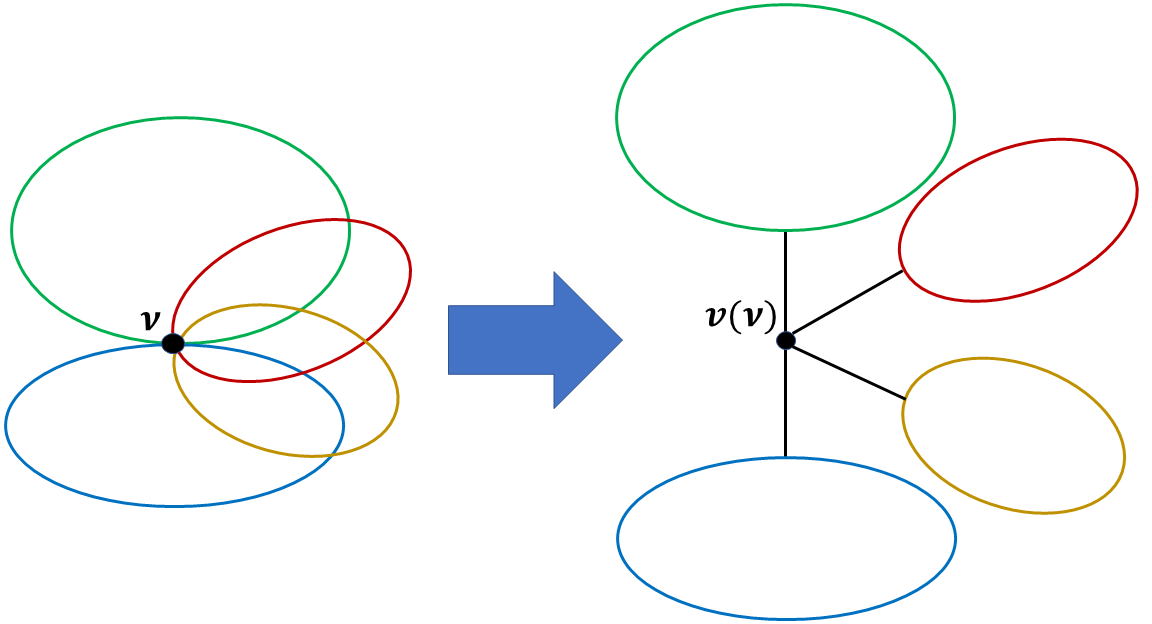
\includegraphics[width=0.6\textwidth]{src/images/Cactus-transformation.png}
%     \caption{Transformation of cactus ${\cal H}_V$ to the tree $T({\cal H}_V)$.}
% \label{fig:transform-cactus-to-tree}
% \end{figure}

% We know that if $\nu$ and $\mu$ are two nodes in the cactus, there exists a unique path of cycles and tree edges between them. It follows from the construction of $T({\cal H}_V)$ that the unique path between the vertices $v(\nu)$ and $v(\mu)$ captures the same path. Thus we state the following lemma.

% \begin{lemma}
% Let $\nu,\mu$ be any two arbitrary nodes in the cactus 
% ${\cal H}_V$. The unique path between $v(\nu)$ and $v(\mu)$ in $T({\cal H}_V)$ concisely captures all
% paths between $\nu$ and $\mu$ in ${\cal H}_S$.
% \label{lem:path-in-T(H_S)}
% \end{lemma}

% % Let $\nu$ and $\mu$ be any two nodes in skeleton ${\cal H}_S$. If they belong to the same cycle, say $c$, there are two paths between them on the cycle $c$ itself - their union forms the cycle itself. Using the fact that any two cycles in  ${\cal H}_S$ can have at most one common node, it can be seen that these are the only paths between $\nu$ and $\mu$. Using the same fact, if $\nu$ and $\mu$ belong to different cycles, there exists a unique sequence of alternating cycles and nodes $\langle \nu_1,c_1,\ldots,\nu_r,c_r,\nu_{r+1}\rangle $ satisfying the following 2 properties. \begin{itemize}
% %     \item $\nu_1=\nu$, $\nu_{r+1}=\mu$, and for each $1< i\le r$, $\nu_i$ is the unique node common to $c_{i-1}$ and $c_i$.
% %     \item Each path between $\nu$ and $\mu$ can be seen as a sequence $\langle p_1,\ldots p_r\rangle$ such that $p_i$ is a path between $\nu_i$ and $\nu_{i+1}$ on cycle $c_{i}$.
% % \end{itemize}
% % It follows from the construction of $T({\cal H}_S)$ that $\langle v(\nu_1),v(c_1),\ldots,v(\nu_r),v(c_r),v(\nu_{r+1})\rangle$ is the path between $v(\nu)$
% % and $v(\mu)$. 
% % Thus we can state the following lemma.
% % \begin{lemma}
% % Let $\nu,\mu$ be any two arbitrary nodes in the cactus 
% % ${\cal H}_S$. The unique path between $v(\nu)$ and $v(\mu)$ in $T({\cal H}_S)$ concisely captures all
% % paths between $\nu$ and $\mu$ in ${\cal H}_S$.
% % \label{lem:path-in-T(H_S)}
% % \end{lemma}

% We root the tree $T({\cal H}_V)$ at any arbitrary vertex and augment it suitably so that it can answer any LCA query in $\mathcal O(1)$ time using \cite{DBLP:journals/jal/BenderFPSS05}. Henceforth, we shall use skeleton tree $T({\cal H}_S)$ to denote this data structure.

% \subsubsection*{Extendability of Proper Paths}
% A \textit{proper path} in a skeleton refers to a path in the skeleton which contains at most one structural edge from a cycle. It is easy to observe that there is at most one proper path between a pair of nodes in the skeleton. We describe a transitive relation between proper paths on skeleton called \textit{extendable in a direction}.


% % {\color{red} extendable in direction $\nu_2$ looks a bit. Try to redefine only in terms of projection mapping paths.}
% % \subsubsection{Extendable in a direction}
% \begin{definition}[Extendable in a direction]
% % Suppose $u$ and $v$ are two stretched units projected to proper paths $P(\nu_1,\nu_2)$ and $P(\nu_3,\nu_4)$ respectively. $v$ is said to be extendable in direction $\nu_2$ of $u$ if proper paths $P(\nu_1,\nu_2)$ and $P(\nu_3,\nu_4)$ are extendable to a proper path $P(\nu,\nu')$ with $P(\nu_1,\nu_2)$ as the initial part and $P(\nu_3,\nu_4)$ as the final part.
% Consider two proper paths $P_1 = P(\nu_1,\nu_2)$ and $P_2 = P(\nu_3,\nu_4)$. $P_2$ is said to be extendable from $P_1$ in direction $\nu_2$ if proper paths $P_1$ and $P_2$ are extendable to a proper path $P(\nu,\nu')$ with $P_1$ as the initial part and $P_2$ as the final part.
% \label{def:extendable}
% \end{definition}

% It follows from Theorem \ref{lem:path-extendable} that if the stretched unit $v$ is reachable from $u$ in the direction $\nu_2$ through a coherent path, then $v$ is extendable in direction $\nu_2$ from $u$.

% It is interesting to note that verifying if $P(\nu_3,\nu_4)$ is extendable from $P(\nu_1,\nu_2)$ in direction $\nu_2$ can be done in ${\cal O}(1)$ LCA queries on the skeleton tree.

% \section{Proof of Lemma \ref{lem:AUB-contains-E_y}} \label{appendix:AUB-contains-E_y}
% \begin{proof}
% It follows from Lemma \ref{lem:3-vertex-lemma}(3) that $A\cup B$ will be a $(s,t)$-mincut. Hence $A\cup B$ will be a transversal in strip ${\cal D}_{A,t}$ that stores all
% $(s,t)$-mincuts.
% From definition, $y$ belongs to $\bar{A}$. Refer to Figure \ref{fig:non-S-crossing}($ii$).  If $y\in \bar{A}\cap B$, then it follows from Lemma \ref{lem:3-vertex-lemma}(1) that all neighbors of $y$ corresponding to $E_y$ will belong to $\bar{A}\cap \bar{B}$. So $E_y$ belongs to the cut defined by $A\cup B$. The same holds for the case $y\in \bar{A}\cap\bar{B}$ as well since $B\subset A\cup B$.
% \end{proof}

\section{Proof of Lemma \ref{lem:s-t-mincut-containing-x-y-topological-fixed}}\label{appendix:s-t-mincut-containing-x-y-topological-fixed}
\begin{proof}
Consider $u \in X$ to be a non-terminal in strip ${\cal D}_{s,t}$. We shall show that ${\cal R}_s(u) \setminus \mathbf{s} \subseteq X$, i.e. reachability cone of $u$ towards source ${\mathbf s}$ in the strip ${\cal D}_{s,t}$ avoiding $\mathbf s$ is a subset of $X$. Consider any non-terminal $v \in {\cal R}_s(u) \setminus \mathbf{s}$. Since $u$ is reachable from $v$ in direction $\mathbf t$, therefore $\tau(v) < \tau(u)$. Therefore, $v \in X$. Therefore, ${\mathbf s} \cup X$ defines a transversal in the strip ${\cal D}_{s,t}$ (from Lemma \ref{lem:mincut-transversal}) and thus defines a $(s,t)$-mincut. The fact that $(x,y)$ lies in this $(s,t)$-mincut follows from the fact that $\tau(y) > \tau(x)$ and thus, $y \not \in X$.
\end{proof}


\section{Proof of Lemma \ref{lem:contracted-subcactus-mincut}} \label{appendix:contracted-subcactus-mincut}

Let $c$ be any cycle (or tree edge) passing through (incident on) $\nu$ in the skeleton
${\cal H}_S$. Let ${\cal D}_{s,t}$ be the strip corresponding to the sub-bunch defined by the structural edge(s) incident on $\nu$ by $c$.
Let $\nu$ be on the side of the source $\mathbf{s}$ in this strip.
Let ${\cal H}_S(c)$ be the subcactus formed by removing the structural edge(s) from $c$ incident on $\nu$ and not containing $\nu$. 
Recall that the subcactus ${\cal H}_S(c)$ was contracted into a vertex, say $v_c$, in the graph 
$G_{S'}$.
%Moreover, suppose $v_c$ is the contracted vertex corresponding to contracted subcactus ${\cal H}_S(c)$.
%Also, assume that $\nu$ is on the side of the source $\mathbf{s}$ in this sub-bunch.

\begin{lemma}
Let $u$ and $u'$ be any two non-terminal units in ${\cal D}_{s,t}$ such that none of them is compressed to $v_c$ in $G_{S'}$. If one of them is reachable from the other in the direction of ${\mathbf{s}}$, then both of them will be compressed to the same contracted vertex in $G_{S'}$.
%
%Let $u$ and $u'$ be any two non-terminal units in ${\cal D}_{s,t}$ such that $u'$ is reachable from $u$ in the direction of ${\mathbf{s}}$ and $u$ is not contracted to vertex $v_c$. $u'$ and $u$ will be compressed to the same contracted node in $G_{S'}$.
\label{lem:u-u'-in-G-nu}
\end{lemma}
\begin{proof}
Assume without loss of generality that $u'$ is reachable from $u$ in the direction of ${\mathbf{s}}$.
Let the proper paths associated with each of $u$ and $u'$ in ${\cal H}_S$ be $P(\nu_1,\nu_2)$ and $P(\nu_1',\nu_2')$ respectively. 
It follows from the construction of ${\cal D}_{s,t}$ that
$P(\nu_1,\nu_2)$ as well as $P(\nu_1',\nu_2')$ will pass through one of the structural edge(s) from $c$ on $\nu$. Without loss of generality,  assume that $P(\nu_1,\nu_2)$ passes through $e$. Since $P(\nu_1,\nu_2)$ is a proper path, this implies that this is the only structural edge in this cut (of skeleton) through which this path passes.
Since $u'$ is reachable from $u$ in flesh ${\cal F}_S$, so $P(\nu_1',\nu_2')$ will also have to pass through $e$ (from Lemma \ref{lem:path-extendable}).
It again follows from Lemma \ref{lem:path-extendable}, that $P(\nu_1,\nu_2)$ as well as $P(\nu_1',\nu_2')$ are subpaths of a path, say $P(\nu',\nu'')$, in skeleton
${\cal H}_S$. This combined with the above discussion establishes that $P(\nu',\nu'')$ has the structure shown in Figure \ref{fig:structure-of-p(nu',nu'')}.

Observe that any path in skeleton that passes through a node $\nu$ can intersect at most 2 cycles or tree-edges that are passing though $\nu$. We know that suffix of $P(\nu',\nu'')$ after $e$ lies in ${\cal H}_S(c)$, so the prefix upto $e$ must have endpoint in subcactus ${\cal H}_S(c')$ where $c'\neq c$. This implies that $u$ must be compressed to $v_{c'}$ because it is not compressed to $v_c$. Thus, $c'$ precedes $c$ in total order. It follows from the structure of path $P(\nu_1',\nu_2')$ that it will have an endpoint in ${\cal H}_S(c')$. Thus, $u'$ will be compressed to the same compressed vertex $v_{c'}$ in $G_{S'}$. This completes the proof.

\begin{figure}%[H]
\centering
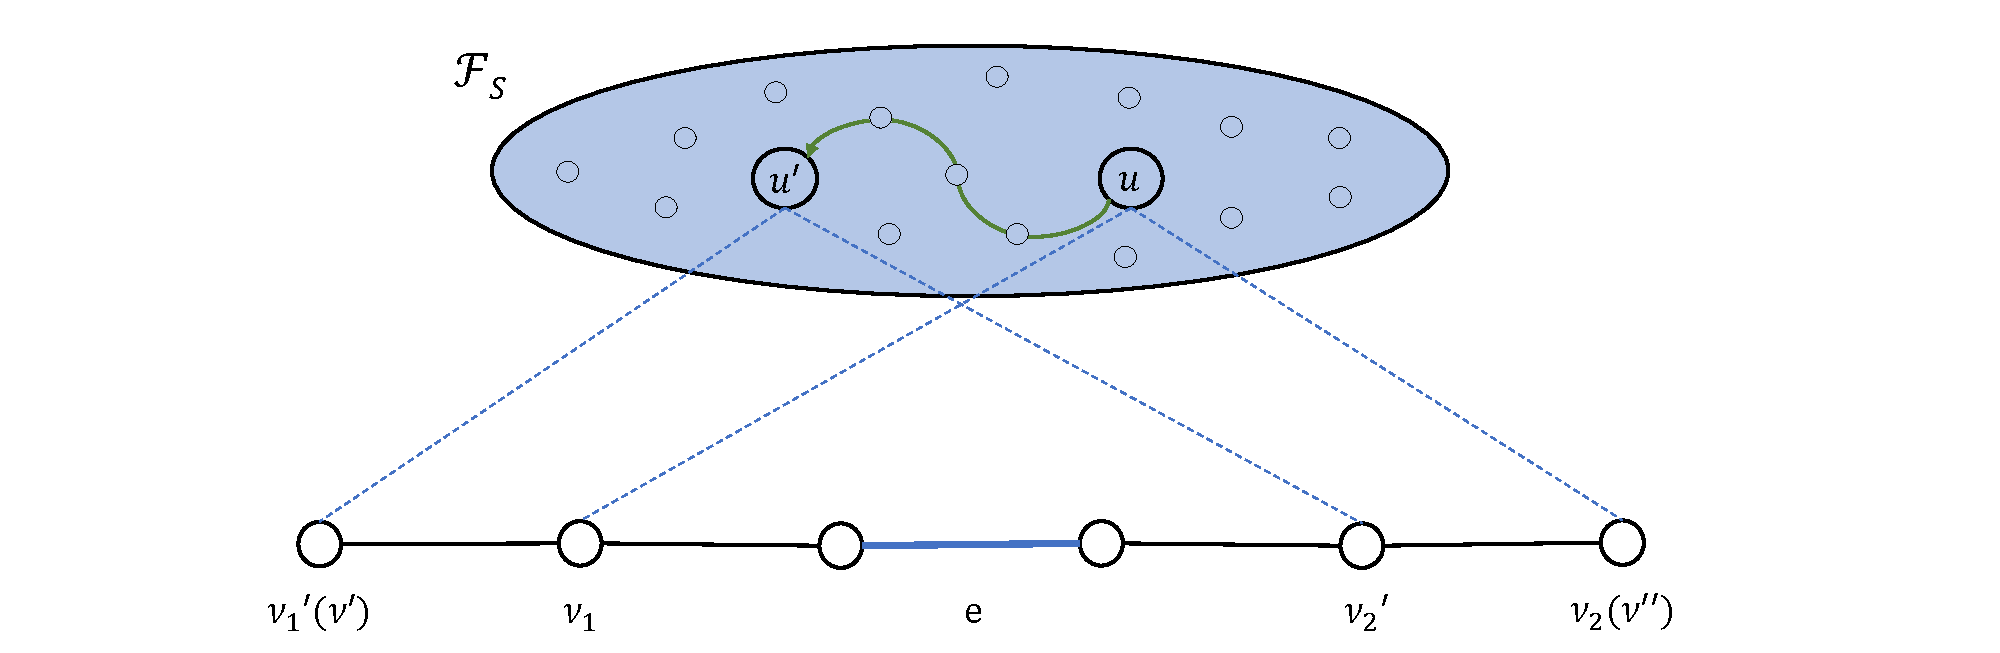
\includegraphics[width=0.95\textwidth]{src/images/proof-reachability-compressed.pdf}
    \caption{The structure of path $P(\nu',\nu'')$.}
\label{fig:structure-of-p(nu',nu'')}
\end{figure}

\end{proof}
% Lemma \ref{lem:contracted-subcactus-mincut} implies that vertex set compressed to each contracted node defines a Steiner mincut. This completes the proof of Lemma \ref{lem:u-u'-in-G-nu}.

Consider the set of non-terminals in the strip ${\cal D}_{s,t}$ that are not compressed to contracted vertex $v_c$. Let this set be $U$. Observe that the set of units $\bigcup_{u\in U} {\cal R}_s(u)$ form a Steiner mincut (using Lemma \ref{lem:reachability-cones}). Moreover, it follows from Lemma \ref{lem:u-u'-in-G-nu} that each non-terminal unit in the set $\bigcup_{u\in U} {\cal R}_s(u)$ is not compressed to contracted vertex $v_c$. Thus, $U = \bigcup_{u\in U} {\cal R}_s(u) \setminus \{\mathbf{s}\}$. All the set of vertices compressed to $v_c$ forms the complement of set $\bigcup_{u\in U} {\cal R}_s(u)$, and thus defines the same Steiner mincut. Therefore, the set of vertices corresponding to each contracted vertex defines a Steiner mincut.

It follows from the construction that $G_{S'}$ is a quotient graph of $G$. Moreover, the number of contracted vertices equals the number of cycles and tree edges incident on node $\nu$ in the skeleton. Figure \ref{fig:image-contraction} gives a nice illustration of the contraction procedure.

\begin{figure}
    \centering
    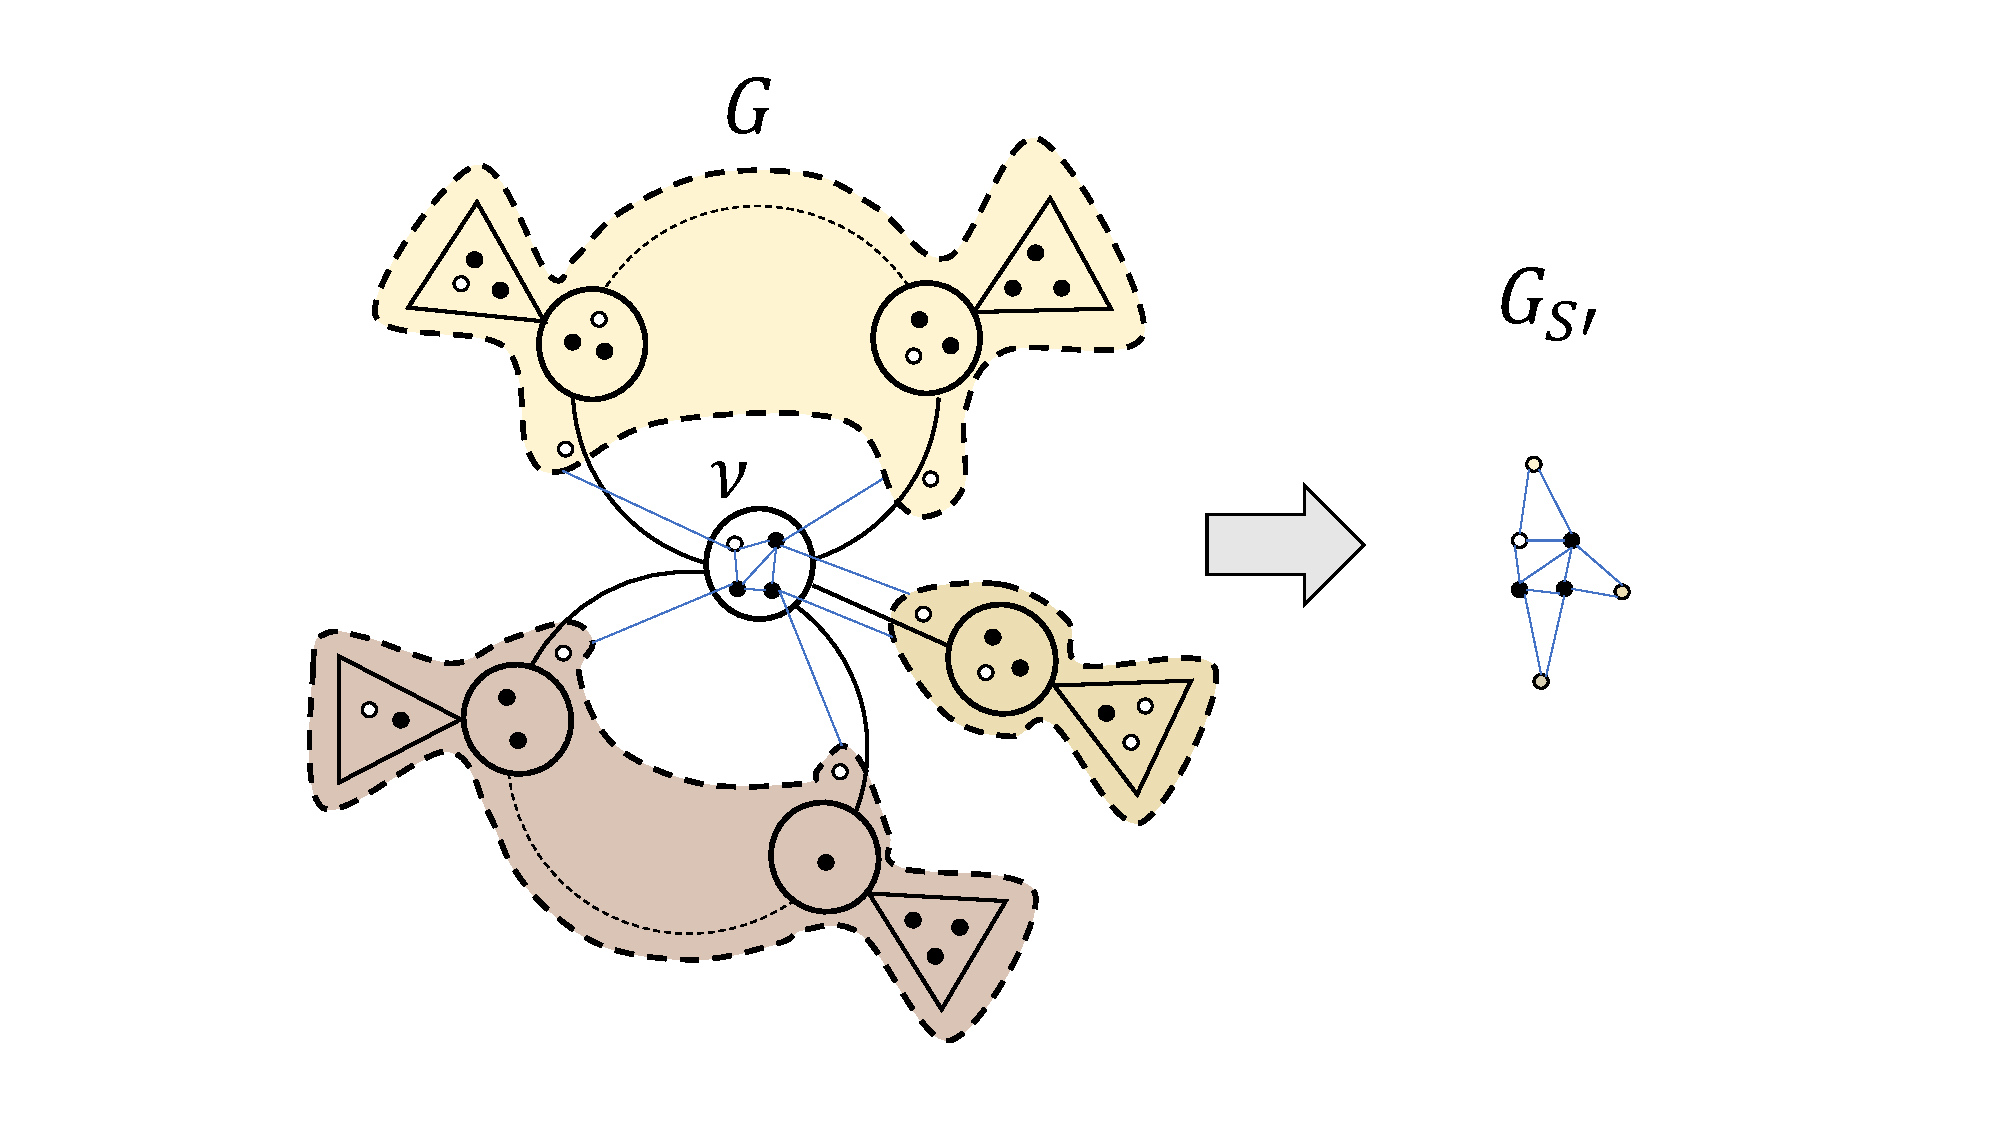
\includegraphics[width=0.9\textwidth]{src/images/image_contraction.pdf}{}
    \caption{$2$-step contraction procedure to construct $G_{S'}$. We only show the vertices and relevant edges of graph along with the skeleton ${\cal H}_S$. Solid vertices belong to Steiner set $S$ and hollow vertices are non-Steiner vertices. All Steiner vertices inside node $\nu$ form the set $S'$.}
    \label{fig:image-contraction}
\end{figure}

\section{Proof of Lemma \ref{lem:linear-time-qt} and \ref{lem:mincut-qt}}
\label{appendix:linear-time-qt}
\begin{proof}
Consider the case when $y$ does not belong to any contracted vertex. In this case, all edges in $E_y$ remain intact in $G_{S'}$ and thus $E_{y'}=E_{y}$.

Now, suppose $y$ belong to contracted vertex $y'$. Let $\bar A$ be the set of vertices compressed to contracted vertex $y'$. We select a vertex $t\in {\bar A} \cap S$ and construct the ${\cal D}_{A,t}$ strip using the flesh ${\cal F}_S$ and skeleton ${\cal H}_S$ in time linear in the size of flesh (using Lemma \ref{lem:strip-from-carcass}). Using the construction outlined in Lemma \ref{lem:query-transformation} we can obtain the set of edges $E_{A}$ by computing reachability cone(s) in strip ${\cal D}_{A,t}$. This takes time linear in size of ${\cal D}_{A,t}$. All edges in $E_A$ share same endpoint $y'$ in $G_{S'}$. Thus, we get the set of edges $E_{y'}$ which is simply all edges in $G_{S'}$ corresponding to set $E_A$. Clearly, this process can be accomplished in time linear in the size of flesh ${\cal F}_S$.

Suppose we have a $(r,s)$-mincut in $G_{S'}$, say $B$ such that $s,t \not\in B$ that contains all edges in $E_{y'}$. If $y$ does not belong to any contracted vertex, this cut itself can be reported as $E_y=E_{y'}$. Suppose $y$ belong to contracted vertex $y'$. We can construct another $(r,s)$-mincut $B\cup R$ (recall the definition of $R$ in Proof of Lemma \ref{lem:query-transformation}). This procedure also involves construction of ${\cal D}_{A,t}$ strip and computation of reachability cone(s) in this strip. This process can also be accomplished in time linear in the size of flesh ${\cal F}_S$.
\end{proof}

% \section{An ${\cal O}(n^2)$ data structure for single edge-containment queries} \label{appendix:n2-ds}

% % We build our ${\cal O}(n^2)$ data structure by augmenting each internal node $\nu$ of hierarchy tree ${\cal T}_G$ with the skeleton ${\cal H}_{S(\nu)}$ and projection mapping $\pi_{S(\nu)}$.

% % Let $s,t$ be any two vertices such that $\nu$ is their LCA in ${\cal T}_G$. $s$ and $t$ must belong to different nodes in the the skeleton ${\cal H}_{S(\nu)}$ stored at $\nu$. Interestingly, the skeleton ${\cal H}_{S(\nu)}$ and the corresponding projection mapping $\pi_{S(\nu)}$ have sufficient information to infer whether any edge $(x,y)\in E$ belongs to some $(s,t)$-mincut. 
% Suppose $S$ is a designated Steiner set and $s,t\in S$ are Steiner vertices separated by some Steiner mincut. We can determine if an edge $(x,y)\in E$ belongs to some $(s,t)$-mincut using the strip ${\cal D}_{s,t}$ that can be built from the connectivity carcass. However, the construction of strip requires ${\cal O}(\min(m,nc_S))$ time. Interestingly, we show that only the skeleton and the projection mapping of the connectivity carcass are sufficient for answering this query in constant time. Moreover, the skeleton and the projection mapping occupy only ${\cal O}(n)$ space compared to the ${\cal O}(\min(m,nc_S))$ space occupied by the entire connectivity carcass.


% Similar to the projection mapping of the stretched units, Dinitz and Vainshtein \cite{DBLP:journals/siamcomp/DinitzV00} introduced the notion of projection mapping for edges as follows. Suppose $(x,y)\in E$. If $x$ and $y$ belong to the same unit, then $P(x,y) = \varnothing$. If $x$ and $y$ belong to distinct terminal units mapped to nodes, say $\nu_1$ and $\nu_2$, in the skeleton ${\cal H}_S$, then $P(x,y) = P(\nu_1,\nu_2)$. If at least one of them belongs to a stretched unit, $P(x,y)$ is the extended path defined in Lemma \ref{lem:path-extendable}. This allows us to state the following lemma which follows from the construction of a strip corresponding to a subbunch given in Section \ref{subsec:connectivity-carcass}.

% % \begin{lemma}[\cite{DBLP:conf/stoc/DinitzV94}]
% % Edge $(x,y)\in E$ appears in the strip corresponding to a subbunch if and only if one of the structural edge in the cut of ${\cal H}_S$ corresponding to this subbunch lies in $P(x,y)$.
% % \label{lem:edge-path-intersect-subbunch}
% % \end{lemma}

% We state the necessary and sufficient condition for an edge $(x,y)$ to lie in an $(s,t)$-mincut. Note that two paths are said to intersect in the skeleton if the unique path of cycle and tree edges in both the paths intersect at some cycle or tree edge.
% % The skeleton ${\cal H}_{S(\nu)}$ and the corresponding projection mapping $\pi_{S(\nu)}$ have the sufficient information to infer whether any edge $(x,y)\in E$ belongs to some $(s,t)$-mincut as stated by the following lemma. We say that two paths intersect if the unique path of cycle and tree edges in both the paths intersect at some cycle or tree edge.

% % \begin{lemma} \label{lem:path-intersects-tree}
% %  Edge $(x,y)\in E$ belongs to a $(s,t)$-mincut if and only if the proper path $P(x,y)$ intersects a path between the nodes containing $s$ and $t$ in in $\mathcal H_{S}$.
% % \end{lemma}
% \begin{proof}
% Observe that an edge $(x,y)$ lies in a $(s,t)$-mincut if and only if it appears in the strip ${\cal D}_{s,t}$ (follows from Lemma \ref{lem:E_y-edges-same-side}). Infact, we can extend this notion for subbunch as well. The edge $(x,y)$ lies in some $(s,t)$-mincut if and only if it appears in the strip corresponding to some subbunch that separates $s$ from $t$.

% Consider each subbunch that separates $s$ from $t$. Let $\nu_1$ and $\nu_2$ be the nodes in ${\cal H}_S$ containing $s$ and $t$ respectively. A cut in ${\cal H}_S$ corresponding to any tree-edge (or pair of cycle edges in same cycle) in the path from $\nu_1$ to $\nu_2$ defines a subbunch separating $s$ from $t$. Moreover, it follows from the structure of the skeleton that no other cut in the skeleton corresponds to a subbunch separating $s$ from $t$. 

% Suppose $(x,y)$ lies in some $(s,t)$-mincut. Thus, it must be in some subbunch separating $s$ from $t$. From the above discussion, we know that this subbunch must correspond to a cut in the path from $\nu_1$ to $\nu_2$ in skeleton ${\cal H}_S$. Moreover, it follows from Lemma \ref{lem:edge-path-intersect-subbunch} that $P(x,y)$ contains one of the structural edge in this cut. This implies that $P(x,y)$ intersects the path from $\nu_1$ to $\nu_2$ in skeleton ${\cal H}_S$.

% Now, consider the other direction of this proof. Suppose $P(x,y)$ and the path from $\nu_1$ to $\nu_2$ intersect at some cycle (or tree edge) $c$. Let $e_1$ and $e_2$ be structural edges belonging to the cycle $c$ that are part of $P(x,y)$ and path from $\nu_1$ to $\nu_2$ respectively (in the case of tree edge $e_1=e_2=c$). Consider the cut in the skeleton corresponding to structural edges $e_1$ and $e_2$. It follows from Lemma \ref{lem:edge-path-intersect-subbunch} that $(x,y)$ lies in the strip corresponding to this subbunch. Since this cut separates $\nu_1$ from $\nu_2$ in ${\cal H}_S$, therefore the subbunch separates $s$ from $t$.
% \end{proof}

% We build our data structure using the findings of Lemma \ref{lem:path-intersects-tree}. We augment each internal node $\mu$ of the hierarchy tree ${\cal T}_G$ with the skeleton tree $T({\cal H}_{S(\mu)})$ and the projection mapping ${\pi}_{S(\mu)}$ corresponding to Steiner set $S(\mu)$. Since augmentation at each internal node takes ${\cal O}(n)$ space, therefore the total space occupied by the data structure is only ${\cal O}(n^2)$.


% % Consider any node $\nu$ in ${\cal T}_G$.
% % Let $s,t$ be any two vertices such that
% % $\nu$ is their LCA in ${\cal T}_G$. $s$ and $t$ must belong to different nodes in the the skeleton ${\cal H}_{S(\nu)}$ stored at $\nu$. 
% % It follows from Lemma \ref{lem:path-intersects-tree} that for a single-edge-containment query, we just have to keep the skeleton tree and the projection mapping at each internal node in ${\cal T}_G$. It is important to note that both these data structures collectively only take up ${\cal O}(n)$ space, contrary to the ${\cal O}(\min(m,nc_S)$ size taken up by the entire connectivity carcass. Thus, the size taken up by complete data structure is only ${\cal O}(n^2)$. 

% Determining whether a given edge belongs to a $(s,t)$-mincut can be done as follows. Let $\mu$ be the LCA of $s$ and $t$ in ${\cal T}_G$. It follows from Observation \ref{obs:(s,t)-mincut-lca} that $c_{s,t}=c_{S(\mu)}$. Thus, $s$ and $t$ must be separated by some Steiner mincut for set $S(\mu)$. We check if paths $P(x,y)$ and $P(\pi_{S(\mu)}(s),\pi_{S(\mu)}(t))$ intersect in the skeleton ${\cal H}_{S(\mu)}$ (using Lemma \ref{lem:path-intersects-tree}). This can be done using ${\cal O}(1)$ LCA queries on the skeleton tree $T({\cal H}_{S(\mu)})$. Since it takes ${\cal O}(1)$ time for answering one LCA query \cite{DBLP:journals/jal/BenderFPSS05}, so the query time will be ${\cal O}(1)$ only. Algorithm \ref{algo:quadratic-space-query} presents a concise pseudocode of the query answering algorithm.

% \begin{algorithm}%[H]
%     \caption{Single edge-containment queries in ${\cal O}(n^2)$ data structure}
%     \label{algo:quadratic-space-query}
%     \begin{algorithmic}[1] % The number tells where the line numbering should start
%         \Procedure{edge-cotained}{$s,t,x,y$}
%             \State{${\mu}\gets$ LCA($\mathcal T_G,s,t$)}
%             \State $\mathcal P_1 \gets P(\pi_{S(\mu)}(s),\pi_{S(\mu)}(t))$
%             \State $\mathcal P_2 \gets P(x,y)$
%             \If{$\mathcal P_1 \cap \mathcal P_2 = \varnothing$} 
%             \State \textbf{return} False
%             \Else 
%             \State \textbf{ return} True
%             \EndIf
%         \EndProcedure
%     \end{algorithmic}
% \end{algorithm}
% We can thus state the following theorem.
% \begin{theorem}
%  Given an undirected graph $G=(V,E)$ on $n=|V|$ vertices, there exists a data structure of 
% ${\cal O}(n^2)$ size that takes ${\cal O}(1)$ time to determine whether an edge $(x,y)\in E$
% belongs to a $(s,t)$-mincut for any $s,t\in V$
% and $(x,y)\in E$.
% \label{thm:O(n^2)-size-data-structure}
% \end{theorem}


\section{Size and Time analysis of compact data structure}
\label{appendix:size-time-analysis-compact-ds}

The data structure doesn't seem to be an ${\cal O}(m)$ size data structure at first sight. Observe that augmentation at any internal node can still take ${\cal O}(m)$ space individually. Interestingly, we show that collective space taken by augmentation at each internal node will still be ${\cal O}(m)$.

We begin with the following lemma which gives a tight bound on the sum of weights of edges in Gomory-Hu tree is $\Theta(m)$. We also give the proof for the same which was suggested in \cite{DBLP:conf/stoc/HariharanKPB07,DBLP:journals/siamcomp/DinitzV00}.

\begin{lemma}[\cite{DBLP:conf/stoc/HariharanKPB07,DBLP:journals/siamcomp/DinitzV00}]
\label{fact:GH-weight}
The sum of weights of all edges in the Gomory-Hu tree is ${\Theta}(m)$.
\end{lemma}
\begin{proof}
Consider any edge $(u,v)\in E$. This edge must be present in every $(u,v)$-mincut. Thus, the sum of weights of all edges in Gomory-Hu tree is at least $m$. Now, root the Gomory-Hu tree at any arbitrary vertex $r$. Let $f$ maps each edge in this tree to its lower end-point. It is easy to observe that $f$ is a one-to-one mapping. Let $e$ be an edge in the Gomory-Hu tree. Observe that $w(e) \leq deg(f(e))$ (where $deg()$ is the degree of vertex in $G$). Thus the sum of weights of all edges in Gomory-Hu tree is at most $2m$. This comes from the simple observation that the sum of the degree of all vertices in $G$ equals $2m$.
\end{proof}

Let us assign each edge $(\mu,\mu')$ in the hierarchy tree ${\cal T}_G$ weight equal to the Steiner mincut value for the Steiner set $S(\mu)$ (if $\mu$ is the parent of $\mu'$). We shall show that sum of the weight of edges in hierarchy tree ${\cal T}_G$ is $\Theta(m)$. %This will help in our analysis later.

To establish this bound refer to algorithm \ref{Construct Tree} that gives an algorithm to construct the hierarchy tree from Gomory-Hu tree. Observe that the variable $ctr$ in this algorithm stores the sum of weights of all edges in ${\cal T}_G$. It is clear that for $k$ edges removed from the Gomory-Hu tree, we add $k+1$ edges of equal weight in ${\cal T}_G$. Thus, the sum of the weight of all edges in ${\cal T}_G$ is at most $4m$ (since $k+1 \leq 2k$). Therefore, we state the following lemma.

\begin{algorithm}%[H]
    \caption{Construct Hierarchy Tree ${\cal T}_G$ from Gomory-Hu Tree $\hat{ \cal T}_{G}$}
    \label{Construct Tree}
    \begin{algorithmic}[1] % The number tells where the line numbering should start
        \State $ctr \gets 0$
        \Procedure{Construct-Tree}{$\hat{ \cal T}_{G}$}
            \If{$\hat{ \cal T}_{G}$ has single node}
            \State Create a node $\mu$
            \State $val(\mu) \gets val(\hat{ \cal T}_{G})$
            \State \textbf{return} $\mu$
            \EndIf
            \State $c_{\min} \gets$ $\min_{e\in \hat{ \cal T}_{G}}w(e)$
            \State Let there be $k$ edges with weight $c_{\min}$
            \State Remove all edges of weight $c_{\min}$ in $\hat{ \cal T}_{G}$ to get $(k+1)$ trees $T_1,..,T_{k+1}$
            \State Create a node $\mu$
            \State $ctr \gets ctr + c_{\min}\times(k+1)$
            \State $children(\mu) \gets \{\textsc{Construct-Tree}(T_i)\;|\;\forall i\in [k+1]\}$
            \State \textbf{return} $\mu$
        \EndProcedure
    \end{algorithmic}
\end{algorithm}

\begin{lemma}
\label{lem:hierarchy-tree-weight}
The sum of weights of all edges in the tree ${\cal T}_G$ is ${\Theta}(m)$.
\end{lemma}
% The size and time analysis of the data structure crucially exploits the following observations,
We shall now give a bound on the size of connectivity carcass augmented at each internal node. The following lemma gives a bound on the size of flesh graph ${\cal F}_S$ for any Steiner set $S$.

\begin{lemma}
Let ${\cal V}_S$ and ${\cal W}_S$ denote the set of Steiner and non-Steiner units respectively in flesh graph ${\cal F}_S$ with Steiner set $S\subseteq V$. The size of ${\cal F}_S$ is bounded by $|{\cal V}_S|c_S + \sum_{u\in {\cal W}_S}deg(u)$.
\label{lem:size-of-flesh}
\end{lemma}
\begin{proof}
Consider the Gomory-Hu tree of the flesh ${\cal F}_S$, say ${\cal T}$. It is evident that the value of mincut between any two units is at most $c_S$. This follows from the definition of a unit. Now, root this tree ${\cal T}$ at some Steiner unit. Let $f$ maps each edge in this tree to its lower end-point. Any edge in this tree has weight at most $c_S$. However, for any non-Steiner unit $u$, $w(f^{-1}(u)) \leq deg(u)$ (where $deg()$ is the degree of vertex in $G$).  Thus, the sum of weight of all edges in ${\cal T}$ is bounded by $|{\cal V}_S|c_S + \sum_{u\in {\cal W}_S}deg(u)$. Using Lemma \ref{fact:GH-weight}, it follows that size of flesh ${\cal F}_S$ is bounded by $|{\cal V}_S|c_S + \sum_{u\in {\cal W}_S}deg(u)$.
\end{proof}

Consider the flesh graph ${\cal F}_{S(\mu)}$ stored at some internal node $\mu$ in the tree. Let ${\cal V}_{S(\mu)}$ and ${\cal W}_{S(\mu)}$ denote the set of Steiner and non-Steiner units respectively in ${\cal F}_{S(\mu)}$. Let $u$ be some non-Steiner unit in ${\cal F}_{S(\mu)}$. It is evident that $u$ consists of only contracted vertices (obtained after the contraction procedure at some ancestral node). This non-Steiner unit gets compressed to a new contracted vertex in all descendants, and in a sense, disappears. Thus, each contracted vertex appears in at most one non-Steiner unit. 

Now, we shall count the total number of contracted vertices introduced at each internal node. We know that this count is an upper bound on the total number of non-Steiner units across all flesh graphs. It follows from Lemma \ref{lem:contracted-subcactus-mincut} that the number of contracted vertices introduced by node $\mu$ to the graph $G_{\mu'}$ associated with its child $\mu'$ is equal to the number of cycles and tree edges incident on node corresponding to $\mu'$ in skeleton ${\cal H}_{S(\mu)}$. We sum this number for each child of $\mu$. The total number of contracted vertices introduced by internal node $\mu$ to all its children is at most twice the number of tree and cycle edges. Since the skeleton is a cactus graph, thus the number of tree and cycle edges is ${\cal O}(|{\cal V}_{S(\mu)}|)$. Moreover, we know that the number of Steiner units in ${\cal F}_{S(\mu)}$ also equals the number of children of node $\mu$ in tree ${\cal T}_G$. Therefore, the number of Steiner units across all flesh graphs stored at each internal node is given by ${\sum}_{\mu \in {\cal T}_G}|{\cal V}_{S(\mu)}|$ which is ${\cal O}(n)$. Thus, the total number of non-Steiner units across all flesh graphs is also ${\cal O}(n)$.

Now, we shall bound the sum of the degree of all non-Steiner units across all flesh graphs. Since each contracted vertex appears in at most one non-Steiner unit, we can sum the degree of all contracted vertices to get an upper bound. It again follows from Lemma \ref{lem:contracted-subcactus-mincut} that the degree of contracted vertex introduced by node $\mu$ is exactly $c_{S(\mu)}$. Thus, the sum of degree of all contracted vertices introduced by node $\mu$ is ${\cal O}(|{\cal V}_{S(\mu)}|c_{S(\mu)})$.

Combining the above observations, we can infer the following.


\begin{inference}
\label{inf:units-O(n)}
The total number of units across all flesh graphs is ${\cal O}(n)$.
\end{inference}
\begin{inference}
\label{inf:sum-degree}
The sum of degree of non-Steiner units across all flesh graphs stored at each internal node $\mu$ is ${\cal O}(\sum_{\mu \in {\cal T}_G}{|{\cal V}_{S(\mu)}|}c_{S(\mu)})$ i.e ${\cal O}(m)$ (follows from Lemma \ref{lem:hierarchy-tree-weight}). In other words, $\sum_{\mu \in {\cal T}_G} \sum_{u \in {\cal W}_{S(\mu)}}deg(u)$ is ${\cal O}(m)$.
\end{inference}


\subsubsection*{Size analysis of Data Structure}
Combining Lemma \ref{fact:GH-weight}, Lemma \ref{lem:hierarchy-tree-weight}, Lemma \ref{lem:size-of-flesh} and Inference \ref{inf:sum-degree} we get the following result.
\begin{equation*}
    \begin{split}
        \nonumber
        \sum_{\mu \in {\cal T}_G}|{\cal F}_{S(\mu)}| &\leq c_1 \times \sum_{\mu \in {\cal T}_G} (|{\cal V}_{S(\mu)}|c_{S(\mu)} + \sum_{u\in {\cal W}_{S(\mu)}}deg(u))\\
        &\leq c_2 \times m
    \end{split}
\end{equation*}


\subsubsection*{Time analysis of Data Structure}

A trivial bound on the query time follows from the size analysis itself. Since the combined size of our data structure is ${\cal O}(m)$, it follows that the sum of sizes of all flesh graphs from the root node to $LCA(s,t)$ will also be ${\cal O}(m)$. Dinitz and Vainshtein \cite{DBLP:conf/stoc/DinitzV94} showed that size of flesh graph ${\cal F}_S$ is ${\cal O}(\tilde{n}c_S)$ for Steiner set $S$, where $\tilde{n}$ is the number of units in the flesh graph. Total number of units across all flesh graphs is only ${\cal O}(n)$ (Inference \ref{inf:units-O(n)}). The value of Steiner mincut increases as we traverse from the root towards a leaf. Thus, $c_{s,t}$ is the maximum Steiner mincut value in the path from root node to $LCA(s,t)$ . Thus, the sum of sizes of all flesh graphs in this path is bounded by ${\cal O}(nc_{s,t})$. Thus, the query time we achieve is ${\cal O}(\min(m,nc_{s,t}))$.


\subsubsection*{Details of projection mapping}

We have shown that combined size of flesh graphs stored at each internal node in hierarchical tree is ${\cal O}(m)$ and the total number of units across them is ${\cal O}(n)$.

In this subsection, we show how to store the exact projection mapping for each flesh unit in our data structure without affecting the ${\cal O}(m)$ size bound achieved in previous subsection. One natural starting point is to inherit mapping of flesh units from the parent. More specifically, if $\nu$ is a child of $\mu$ in the hierarchy tree, ${\cal F}_\nu$ inherits its mapping from ${\cal F}_\mu$. However, this simple approach may blow up the size of data-structure to ${\cal O}(n^2)$. The way we perform the mapping is as follow, whenever a new contracted vertex is introduced at internal node $\mu$ we map it directly to the stretched unit it appears in any subsequent levels. Note that it might be possible that such a contracted vertex never appears in any stretched units in the subsequent level in which case we map it to the leaf node of the hierarchy tree it finally ends up in. 

Whenever we wish to check if a contracted vertex $v$ is mapped to node $\nu$ in flesh ${\cal F}_\mu$, we go to the mapping of $v$, let it be ${\pi(v)}$. Now, $\pi(v)$ might be a stretched unit corresponding to some internal node or a leaf node itself. Assume the internal node corresponding to $\pi(v)$ is $\nu'$, we lookup the LCA($\nu,\nu'$). If LCA($\nu,\nu'$)$=\nu$, we can conclude that $v$ is mapped to node $\nu$ in this level.

Let us look the query procedure more closely. The query procedure shall be of the form \textsc{edge-contained}$(s,t,E_y)$ at any internal node $\mu$ where $s$ and $t$ are vertices of graph and $E_y$ is a set of edges incident on a unit $y$ in the flesh graph ${\cal F}_\mu$. The task at this stage is to understand how to transform this query to the form \textsc{edge-contained}$(s,t,E_{y'})$ for a child node $\nu$ of $\mu$. One of these two cases are possible, ~$(i)$ $y$ is in the unit same as $s,t$ which is mapped to node $\nu$ in the skeleton. In this case, $E_{y'}=E_y$ and $y=y'$, so we need not do anything. ~$(ii)$ $y$ is some other unit (not same as $s,t$) in the flesh ${\cal F}_\mu$. Observe that $E_y$ must also be edges in ${\cal F}_\mu$ otherwise the query can be answered in negative. After doing the query transformation, we shall get a set of edges $E_{v}$ where $v$ is a contracted vertex. Thus, we need to identify the unit in ${\cal F}_\nu$ where $v$ lies. How can one do the same? We know that contracted vertices are not mapped to units in flesh ${\cal F}_\nu$ but are directly mapped to the stretched unit (or the leaf node) it ever appears in. So, we can lookup the mapping $\pi(v)$ which will be a stretched unit in flesh ${\cal F}_{\mu'}$ or simply a leaf node $\mu'$. If $\nu = \mu'$, $y'=\pi(v)$. Otherwise, we can't infer directly the steiner unit in which $v$ lies. We perform this simple procedure -- for each Steiner unit we check if $v$ lies in that Steiner unit. We have already seen that the ``check" operation only takes constant time as it can be accomplished using a LCA query on the hierarchy tree. Since, we already discount $|{\cal F}_\nu|$ time for the node $\nu$ in the query procedure, identifying $y'$ does not poses a challenge to query time.


%%%%%%%%%%%%%%%%%%%%%%%%%%%%%| OLD IDEAS START |%%%%%%%%%%%%%%%%%%%%%%%%%%%%%%%%%%%
% \subsection{Making $O(n^2)$ data structure self-sustainable}

% \begin{itemize}
%     \item Count the number of distinct stretched units in the whole data structure. 
    
% The number of new stretched units introduced at a level seems proportional to the number of edges in the skeleton at this level. Thus, the number of distinct stretched units should only be $O(n)$.

%     \item The two partition of a stretched unit if it appears at multiple levels remains same. From the 3-vertex lemma, observe that if $r,s$ are two vertices in source side and $t$ is a vertex on sink side of a strip with $u$ as a stretched/non-terminal unit then any $(r,s)$-mincut preserves the partition of the stretched unit $u$.
% \end{itemize}


% \subsection{Stretched Units in ${\cal O}(n^2)$ data structure}

% Suppose $\nu$ is a node in the skeleton ${\cal H}_S$ and is part of a cycle $C$. We define \texttt{Nearest}($\nu,C$) to be the nearest $\nu$-mincut from the bunch corresponding to the cycle edges of $C$ incident on node $\nu$. To be precise, the units contained in \texttt{Nearest}($\nu,C$) will be those, both endpoints of whose projection mapping, lies in the subcactus formed by removing two edges of cycle $C$ incident on node $\nu$ and containing $\nu$. Overloading this notation, we define \texttt{Nearest}($\nu,e$) for a tree-edge $e$ incident on node $\nu$ in the skeleton. \texttt{Nearest}($\nu,e$) is the nearest $\nu$-mincut from the bunch corresponding to the tree-edge $e$. All units whose both endpoints lies in the  subcactus formed by removing tree-edge $e$ incident on node $\nu$ and containing $\nu$ constitutes the set \texttt{Nearest}($\nu,e$).

% It is important to note that the if ${\cal V}_S$ is the number of steiner units in the flesh ${\cal F}_S$, then the total number of \textit{distinct} sets \texttt{Nearest}($\nu,C$) or \texttt{Nearest}($\nu,e$) for all possible nodes $\nu \in {\cal V}_S$ and cycles $C$ or tree-edges $e$ incident on $\nu$ is only ${\cal O}(|{\cal V}_S|)$. Therefore, if we look at all levels combined, the number of such sets is thus bounded by ${\cal O}(n)$.

% In the remaining section, we shall show that set defined by a stretched unit at any internal node in our hierarchical data structure defines the same set as one of the \texttt{Nearest}($\nu,C$) or \texttt{Nearest}($\nu,e$) sets at some of its ancestral level.


% In this section, we shall have a closer look at the stretched units that are present at different levels of our data structure. Consider any internal node $\nu$ and suppose there is a stretched unit $\bf{u}$ at this level of the data structure. Let $r,s \in S_{\nu}$ be two steiner vertices at this level such that stretched unit $\bf u$ appears in the $(r,s)$-strip. Also, assume $u \in V$ is a vertex mapped to the stretched unit $\bf{u}$. Suppose $\mu$ is the LCA of $\nu$ and $u$. It follows from the construction that $r,s,u \in S_{\mu}$ and $c_{r,u} = c_{s,u} < c_{r,s}$.

% \begin{lemma}
% \label{lem:2-parition-coincides}
% If same stretched unit appears at multiple levels in the hierarchical data structure, its inherent partition coincides in each of them.
% \end{lemma}
% \begin{proof}

% {
% \color{red}

% Extend it to multiple levels from cactus-notes paper.
% }

% Suppose $u$ is a non-terminal unit that appears in two strips corresponding to bunches ${\cal B}$ and ${\cal B}'$. Suppose $(A,{\bar A})$ and $(B, {\bar B})$ be two steiner mincuts that contain one side of the star of $u$ ($u\in A\cap B$) in the strip corresponding to strips ${\cal W}_{\cal B}$ and ${\cal W}_{\cal B'}$ respectively. Moreover, assume that $E_u$ is the star of $u$. Observe that two cases are possible -- either $A\cap B$ contains at least a steiner vertex or it contains none. 


% Consider the case when $A\cap B$ contains a steiner vertex. It follows from 3-vertex lemma that $A\cap B$ must define a steiner mincut. Thus, $c(A\cap B \setminus \{u\}) \leq c(A\cap B)$. A little analysis shows that $c(u, A\cap B \setminus \{u\}) = c(u, {\bar A}\cap {\bar B}) = \frac{|E_u|}{2}$. Thus, $E(u,{\bar A}) = E(u,{\bar B})$. Thus, the two sides of star coincide.

% Now, consider the case when $A\cap B$ has no steiner vertex. It follows from 3-vertex lemma that $E(A\cap B, {\bar A}\cap {\bar B})=\varnothing$ (and hence $E(u,{\bar A}\cap {\bar B})=\varnothing$). Thus, $E(u,{\bar A})\cup E(u, {\bar B}) = E_u$. Moreover, $E(u,{\bar A})\cap E(u, {\bar B}) = \varnothing$. Thus, the two sides of star coincide in this case as well.
% \end{proof}

% We now state an important lemma which conveys the relation between stretched units and skeleton graph that is stored at multiple levels of our hierarchical data structure.

% \begin{lemma}
% \label{lem:stretched-unit-subcactus}
% Each stretched unit stored at an internal node defines the same set of vertices as one of the set \texttt{Nearest}$(\nu,C)$ or \texttt{Nearest}$(\nu,e)$ from one of its ancestral level.
% \end{lemma}
% \begin{proof}
% {
% \color{red} To be done.
% }
% \end{proof}
% An immediate consequence of Lemma \ref{lem:2-parition-coincides} and \ref{lem:stretched-unit-subcactus} is the following corollary.

% \begin{corollary}
% The total number of distinct stretched units across all internal nodes is only ${\cal O}(n)$.
% \end{corollary}

%%%%%%%%%%%%%%%%%%%%%%%%%%%%%%%%%%%%| OLD IDEAS END |%%%%%%%%%%%%%%%%%%%%%%%%%%%%%%%%



%%%%%Important Portion %%%%%%%%%%%%%%%
% \subsection{Strip representation of reachability in directed graphs}

% The problem of reachability in directed graph is as follows -- Given a directed graph $\vv{G}$, preprocess it to form a data structure which can efficiently report if a given vertex $v$ is reachable from another vertex $u$. The problem becomes interesting if we allow the underlying graph to be sparse. Is there any data structure that takes ${o}(n^2)$ space and still offers efficient query time? Patrascu \cite{DBLP:journals/siamcomp/Patrascu11} stated it as a difficult open problem and also gave a partial answer to it. In particular, if constant query time is required, the space needs to be $n^{1+\Omega(1)}$. Goldstein et al \cite{DBLP:conf/wads/GoldsteinKLP17} stated a conjecture that concisely conveys the belief.

% \begin{conjecture}[Directed Reachability Hypothesis \cite{DBLP:conf/wads/GoldsteinKLP17}]
% \label{conj:directed-reachability-hypothesis}
% Any data structure for the problem of reachability in directed graphs must either use ${\tilde \Omega}(n^2)$ space, or linear query time.
% \end{conjecture}

% The reachability in $\vv{G}$ is same as reachability in $G_{SCC}$, a directed acyclic graph which can be obtained by contracting each of the Strongly Connected Components (SCCs) to a single vertex. Henceforth, we shall assume that $\vv{G}$ is a directed acyclic graph.

% We can transform a directed acyclic graph $\vv{G}$ into a $(s,t)$-strip ${\cal D}_{s,t}$ as follows. Create two additional vertices, namely $s$ and $t$. Suppose $\Delta_v$ denotes the difference in indegree and outdegree of any vertex $v$ in $V(\vv{G})$. For each vertex $v \in V(\vv{G})$, if $\Delta_v > 0$ we add $\Delta_v$ edges from $v$ to $t$. Likewise, if $\Delta_v < 0$ we add $|\Delta_v|$ edges from $s$ to $v$. Lastly, add two additional edge(s) from $s$ to $v$ and $v$ to $t$ for all $v \in V(\vv{G})$. Note that the resultant graph is a strip by making all the edges undirected and taking the inedges and outedges as the inherent partition of each non-terminal unit. Moreover, the number of edges in this graph is only ${\cal O}(m)$. A non-terminal unit $v$ is reachable from another non-terminal unit $u$ if and only if there exists a coherent path from $u$ to $v$ in ${\cal D}_{s,t}$.

% \subsection{Conditional Lower Bound for $2-$failure fault-tolerant $(s,t)$-mincut}

% Suppose we wish to determine if a vertex $v$ is reachable from another vertex $u$ in $\vv{G}$. Since, $\vv{G}$ is also a DAG, it may be assumed that $v$ exceeds $u$ in topological order. We show that reachability can be checked using the fault-tolerant query \texttt{ft-mincut}$(s,t,\{(s,u),(v,t)\})$ on the strip ${\cal D}_{s,t}$. $v$ is reachable from $u$ if and only if the fault-tolerant query returns value equal to the original mincut between $s$ and $t$ less unity. In other words, $v$ is reachable from $u$, if and only if \texttt{ft-mincut}$(s,t,\{(s,u),(v,t)\}) = c_{s,t} - 1$. Thus, we state the following conditional lower bound in form of a conjecture.


% \begin{conjecture}
% A $2-$failure fault-tolerant $(s,t)$-mincut data structure with designated pair of vertices $s$ and $t$ must use ${\tilde \Omega}(n^2)$ space if it gives constant query time.
% \end{conjecture}




% \subsection{Fault tolerance for a source-destination pair}
% Let $G=(V,E,c)$ be a directed graph with a designated source vertex $s$, a designated sink vertex $t$, and capacity $c:E\rightarrow R^+$. Let $G_f$ be the residual network corresponding to a maximum ($s,t$)-flow $f$. Note that there is no path from $s$ to $t$ in $G_f$. Let $D_f$ be the SCC graph obtained by contracting each SCC of $G_f$ into a single vertex. Let ${\bf s}$ be the node containing $s$ and ${\bf t}$ be the node containing $t$. Note that $D_f$ is a DAG, and let $\tau$ be any topological numbering of $D_f$ with $\tau({\mathbf t})=k$ and $\tau({\mathbf s})=\ell$. Note that $k<\ell$.  The following lemma states an easy way to identify a $(s,t)$-mincut from $D_f$ using $\tau$. 
% \begin{lemma}
% Let $v$ be any node in $D_f$ such that $k<\tau(v)\le \ell$. The set of nodes in $D_f$  with topological number $\ge \tau(v)$ constitutes a $(s,t)$-mincut in $G$.
% \label{lem:simple-mincut-from-top-number}
% \end{lemma}
% \begin{proof} 
% Let $S$ be the set of nodes of $D_f$
% with topological numbering $\ge \tau(v)$ in $D_f$, and let $A$ be the set of vertices in $G$ that are mapped to the nodes of $S$. First note that $s\in A$ and $t\notin A$, so $A$ defines a ($s,t$)-cut in $G$. Since $D_f$ is a DAG and $\tau$ is a valid topological numbering, there does not exist any edge that originates from a node in $S$ and enters a node outside $S$
% in $D_f$. This has the following implications:
% \begin{itemize}
%     \item 
%     Let $(u,v)$ be an edge in $G$ with $u\in A$ and $v\in V\backslash A$. It follows from the construction that the node containing $v$ must be outside $S$. The flow $f(u,v)$ must be equal to $c(u,v)$; otherwise $(u,v)$ be a forward edge in $G_f$. This edge will appear as emanating from the node containing $u$ to node containing $v$ in $D_f$. In other words, this edge will appear as an edge originating from $S$ and entering a node outside $S$ in $D_f$, which is not possible.
%     \item
%     Let $(u,v)$ be an edge in $G$ with 
%     $v\in A$ and $u\in V\backslash A$. It follows from the construction of $S$
%     that node containing $u$ must be outside $S$.
%     The flow $f(u,v)$ must be zero; otherwise it would imply that $(v,u)$ is a backward edge in $G_f$. This backward edge will appear as an edge originating from $S$ and entering a node outside $S$ in $D_f$, which is not possible.
% \end{itemize}
% Hence all edge leaving $A$ in $G$ are fully saturated and any edge entering $A$ from $V\backslash A$ must not be carrying any flow. Hence $f(A,V\backslash A)$ matches $c(A, V\backslash A)$. Hence $(A,V\backslash A)$ must be a $(s,t)$-mincut.
% \end{proof}

% % We know that given any edge $(x,y)\in E$,
% % we can determine in $O(1)$ time whether $(x,y)$ belongs to any $(s,t)$-mincut in $G$ as follows. 

% % If $x$ and $y$ belong to the same node in
% % $D_f$, then failure of $(x,y)$ does not affect $(s,t)$-mincut. If $x$ and $y$ belong to different nodes in $D_f$, then
% % $(x,y)$ belongs to a $(s,t)$-mincut if and only if $k\le \tau(y) < \tau(x)\le \ell$.

% We can use Lemma \ref{lem:simple-mincut-from-top-number}
% to efficiently report the $(s,t)$-mincut after the deletion of the edge $(x,y)$ as follows.
% \begin{enumerate}
%     \item If $x$ and $y$ belong to the same node in $D_f$, there is no change in $(s,t)$-mincut.
%     \item Let $\mu$ be the node containing $x$ and $\nu$ be the node containing $y$ in $D_f$. $(x,y)$ will belong to a $(s,t)$-mincut if and only if $k\le \tau(\nu)<\tau(\mu)\le \ell$. If it so happens, let $S$ be the set of nodes in $D_f$ with topological numbering $\ge \tau(\mu)$. It follows from Lemma \ref{lem:simple-mincut-from-top-number} that $S$ defines a $(s,t)$-mincut and $(x,y)$ belongs to this mincut.
%  \end{enumerate}
 
 
 
% \subsection{Plan}

% \begin{itemize}
%     \item { \color{blue} Introduction} -- we should mention why this results are good by comparing with reachability problem , i.e. no tradeoff in between is likely.
%     \item { \color{blue} Preliminaries} -- should also contain definition of nearest mincuts. An edge $(u,v)$ insertion increases $(s,t)$-mincut if $u$ and $v$ are in nearest $(s,t)$-mincut and $(t,s)$-mincut respectively.
%     \item { \color{blue} Compact Representation for Mincuts} -- should also contain KKKZ tree storing all-pairs mincut value.
%     \item Lower Bounds for the problem.
%     \item ${\cal O}(n^2)$ space data structure
%     \item { \color{blue} Insights into $3-$vertex mincuts}
%     \item { \color{blue} Compact Graph for Query Transformation for edge deletion} -- add checking if $u$ is in nearest $(s,t)$-mincut (edge-insertion query).
%     \item { \color{blue} ${\cal O}(m)$ space data structure} -- along with edge insertion.
% \end{itemize}